
\documentclass[conference,letterpaper]{IEEEtran}
\usepackage[T1]{fontenc}
\usepackage{mathptmx}
\usepackage{graphicx}
\usepackage{amsmath}
\usepackage{tabularx}
\usepackage{float}
\usepackage{balance}
\usepackage{listings}
\usepackage{url}
\usepackage[hidelinks]{hyperref}
\lstset{basicstyle=\ttfamily\scriptsize,breaklines=true,columns=fullflexible,keepspaces=true,showstringspaces=false,frame=single,framerule=0.2pt,xleftmargin=3pt,xrightmargin=3pt}
\hyphenation{ware-house re-plen-ish-ment}
\begin{document}
\title{International Supply Chain Analytics}
\author{\IEEEauthorblockN{Ankith Ramesh Babu}\IEEEauthorblockA{Independent Operations Analytics Project}}
\maketitle
\thispagestyle{plain}\pagestyle{plain}
\begin{abstract}This paper presents a reproducible order-fulfillment analysis using 1,200 synthetic orders across four warehouse regions. A seeded simulation separates blocked demand, inventory availability and delivery timing, then produces a prioritized exception register and regional scorecards. The baseline contains 106 blocked orders, a 78.57\% unit fill rate on unblocked demand and an 8.92\% on-time-in-full rate. The distinction between overlapping shortage flags and exclusive primary status is made explicit. Offline dashboards, editable Power BI project source and automated checks provide traceable evidence. Results characterize the simulated dataset rather than a deployed logistics operation.\end{abstract}

\begin{IEEEkeywords}supply chain analytics, order fulfillment, OTIF, exception management, reproducibility\end{IEEEkeywords}

\section{Introduction and System Architecture}

\subsection{Questions addressed}

\textbullet{} Which orders require action, and why?


\textbullet{} How much demand can be fulfilled on unblocked orders?


\textbullet{} Which warehouse has the largest exception workload?


\textbullet{} How does the definition of OTIF change interpretation?


\subsection{Processing sequence}

Table~\ref{tab:1} summarizes analysis stages and outputs.

\begin{table}[H]
\caption{Analysis stages and outputs}\label{tab:1}
\centering\footnotesize
\setlength{\tabcolsep}{3pt}
\begin{tabularx}{\columnwidth}{>{\raggedright\arraybackslash}X >{\raggedright\arraybackslash}X >{\raggedright\arraybackslash}X}
\hline
\textbf{Stage} & \textbf{Implementation} & \textbf{Output} \\
\hline
Generate & Seeded Python simulation & Operational records \\
Calculate & Documented business rules & KPIs and decision fields \\
Export & Deterministic CSV / JSON writer & Auditable report files \\
Present & HTML and PBIR visual definitions & Interactive review surfaces \\
Verify & Unit tests, schema and browser checks & Validation evidence \\
\hline
\end{tabularx}
\end{table}

\subsection{Design decisions}

The analysis uses Python standard-library functions to keep execution portable. The browser report embeds its data and needs no server. The Power BI model embeds the same CSV snapshot in Power Query, avoiding machine-specific paths. Data generation and decision rules remain separate from presentation.


\subsection{Operational boundaries}

This is a batch analysis of simulated observations. It does not write to SAP, execute procurement transactions, reserve stock or authorize operational changes. Each exported row retains the identifiers needed to trace a result back to its source observation.


\section{Data specification and provenance}

All source observations are generated in src/run.py with a fixed random seed \cite{r1}. No customer, supplier or employee data is used. Regional names represent four analytical groups, not actual sites.


Table~\ref{tab:2} summarizes source fields and definitions.

\begin{table}[H]
\caption{Source fields and definitions}\label{tab:2}
\centering\footnotesize
\setlength{\tabcolsep}{3pt}
\begin{tabularx}{\columnwidth}{>{\raggedright\arraybackslash}X >{\raggedright\arraybackslash}X >{\raggedright\arraybackslash}X}
\hline
\textbf{Field} & \textbf{Type} & \textbf{Meaning} \\
\hline
order\_id & Text / unique & SO-prefixed order identifier \\
warehouse & Text & Germany, Hong Kong, Taiwan, Malaysia \\
ordered\_units & Integer & Uniformly sampled from 1 to 120 \\
available\_units & Integer & max(0, order quantity + offset -45 to +25) \\
blocked & Boolean & Independent probability of 9\% \\
delivery\_delay\_days & Integer & Uniform integer from -2 to 8 \\
fulfilled\_units & Integer & 0 if blocked, otherwise min(quantity, stock) \\
status / OTIF & Derived & Priority classification and strict delivery flag \\
\hline
\end{tabularx}
\end{table}

The availability field is a per-order snapshot. The simulation does not share inventory between orders or model a rolling stock ledger. Delivery delay is sampled independently of stock and block status. These simplifications create a controlled exception dataset. Seed 42 produces the committed baseline.


\subsection{Traceability}

Committed CSVs, KPI JSON, analysis JSON and the Power BI embedded snapshot refer to the same default run. Changes to seeds or assumptions require regenerated reports and a new result interpretation.


\section{Analytical Methodology}

Table~\ref{tab:3} summarizes metric definitions.

\begin{table}[H]
\caption{Metric definitions}\label{tab:3}
\centering\footnotesize
\setlength{\tabcolsep}{3pt}
\begin{tabularx}{\columnwidth}{>{\raggedright\arraybackslash}X >{\raggedright\arraybackslash}X}
\hline
\textbf{Metric} & \textbf{Definition} \\
\hline
Unit fill rate & Fulfilled units / ordered units on unblocked orders \\
OTIF rate & Unblocked AND full quantity AND delay <= 0, divided by all orders \\
Shortage units & max(ordered units - available units, 0) \\
Status priority & Blocked, then Stock shortage, then Late, then On track \\
\hline
\end{tabularx}
\end{table}

\subsection{Worked example}

An unblocked order requests 10 units with 6 available and a delay of -1 day. Fulfilled quantity is 6, shortage is 4 and the order contributes 60\% unit fill. OTIF is false because the order is incomplete. If the order is blocked, fulfillment becomes zero and its quantity is excluded from the unit-fill denominator.


\subsection{Overlapping flags versus exclusive status}

The baseline contains 753 orders with an availability shortage, but 687 rows carry the primary status Stock shortage. The remaining 66 shortage orders are blocked and therefore receive the higher-priority Blocked status. Counting primary status and counting shortage flags answer different questions.


\subsection{Denominator policy}

OTIF uses all 1,200 orders and therefore includes the operational effect of blocks. Unit fill rate excludes blocked demand to isolate fulfillable, released demand. These two measures must not be treated as interchangeable service measures.


\section{Results and interpretation}

The analysis output is shown in Fig.~\ref{fig:results}.

\begin{figure}[!t]
\centering
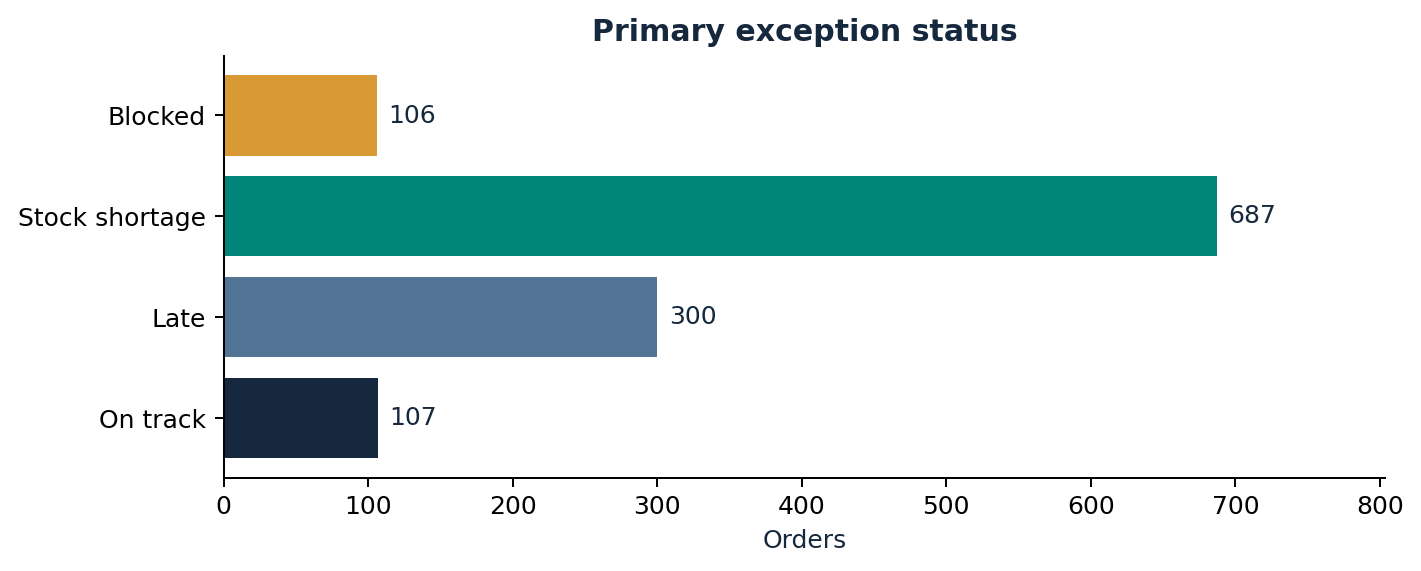
\includegraphics[width=\columnwidth,height=0.25\textheight,keepaspectratio]{../../reports/figures/results.png}
\caption{Baseline results calculated from the committed operational records.}\label{fig:results}
\end{figure}

Table~\ref{tab:4} summarizes regional baseline results.

\begin{table}[H]
\caption{Regional baseline results}\label{tab:4}
\centering\footnotesize
\setlength{\tabcolsep}{3pt}
\begin{tabularx}{\columnwidth}{>{\raggedright\arraybackslash}X >{\raggedright\arraybackslash}X >{\raggedright\arraybackslash}X >{\raggedright\arraybackslash}X}
\hline
\textbf{Warehouse} & \textbf{Orders} & \textbf{Fill rate} & \textbf{OTIF} \\
\hline
Germany & 285 & 79.33\% & 9.47\% \\
Hong Kong & 315 & 78.94\% & 8.89\% \\
Taiwan & 292 & 78.18\% & 7.88\% \\
Malaysia & 308 & 77.86\% & 9.42\% \\
\hline
\end{tabularx}
\end{table}

The main workload is stock shortage: 687 orders carry this primary status. Another 300 complete, unblocked orders are late. Only 107 orders meet the complete, unblocked and on-time condition. The 1,093-row exception register excludes the 107 On track orders.


The low OTIF value follows the deliberately difficult simulation distributions. It is not a benchmark for any company. The practical use is testing whether the exception rules and denominator choices produce an auditable queue.


\section{Interactive dashboard overview}

The dashboard view is shown in Fig.~\ref{fig:dashboard}.

\begin{figure*}[!t]
\centering
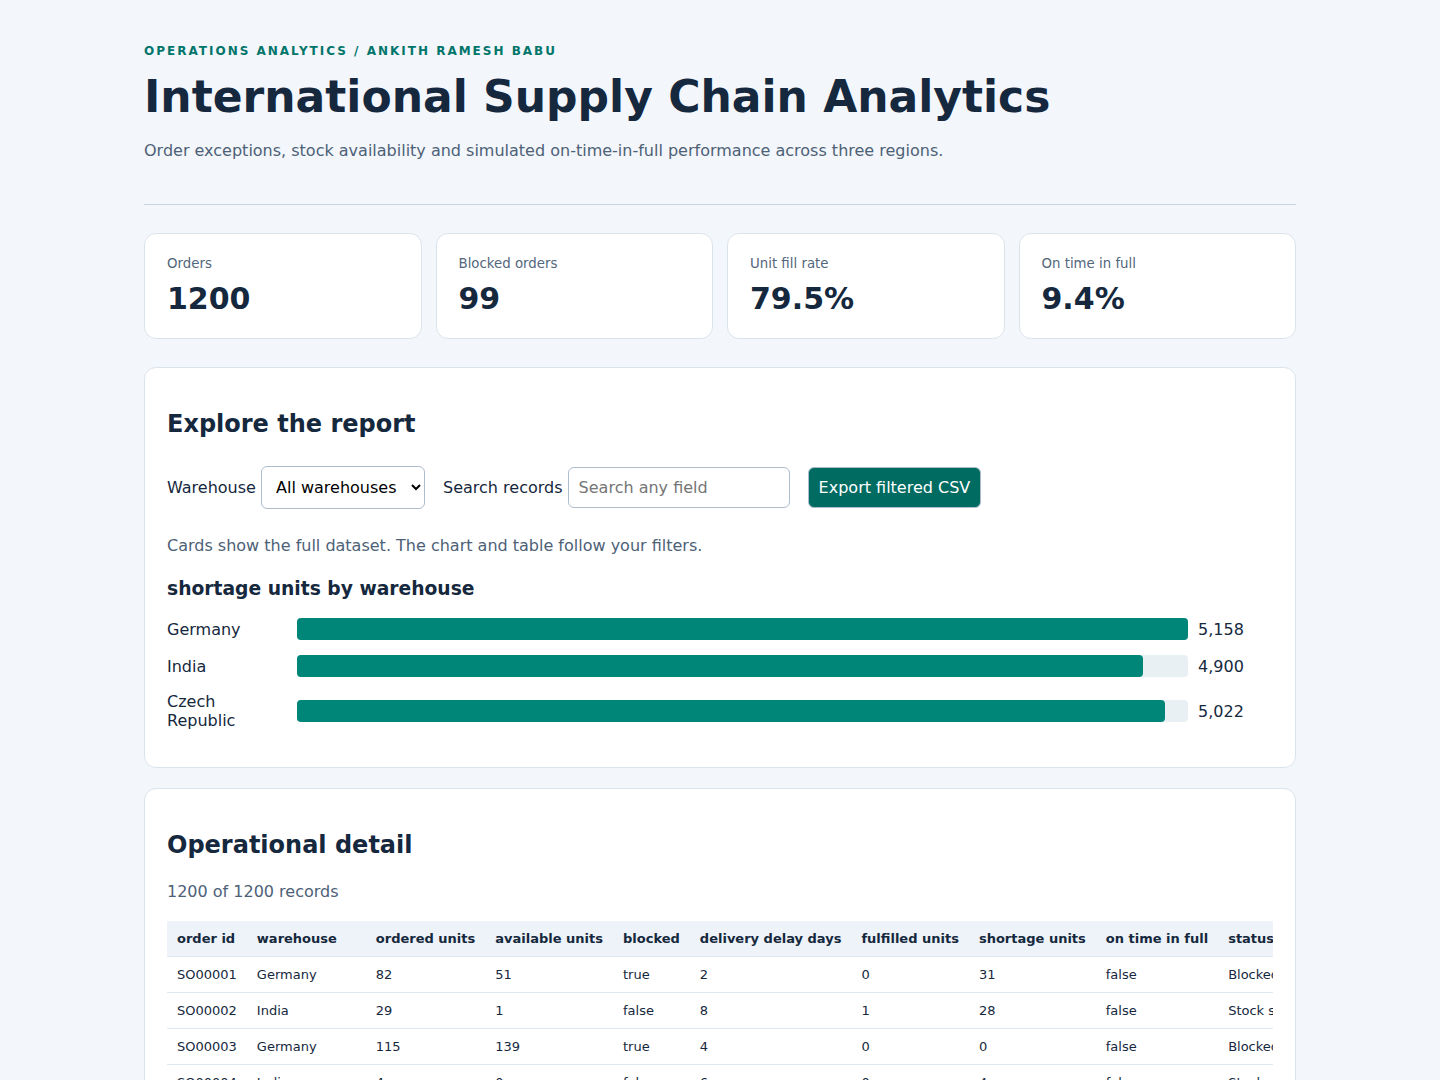
\includegraphics[width=0.90\textwidth,height=0.72\textheight,keepaspectratio]{../../reports/figures/dashboard.png}
\caption{Actual browser capture of the generated HTML dashboard, baseline run.}\label{fig:dashboard}
\end{figure*}

The overview combines full-dataset KPI cards with warehouse filtering, text search, a comparative bar chart and a detailed register. Its data is embedded in the HTML, so the report opens offline without account access.


Display precision differs from the calculation exports: the HTML KPI cards show one decimal place for ratios, while KPI JSON preserves four decimal places. This is display rounding, not a calculation difference.


\section{Dashboard interaction and audit trail}

The dashboard view is shown in Fig.~\ref{fig:dashboard-germany}.

\begin{figure*}[!t]
\centering
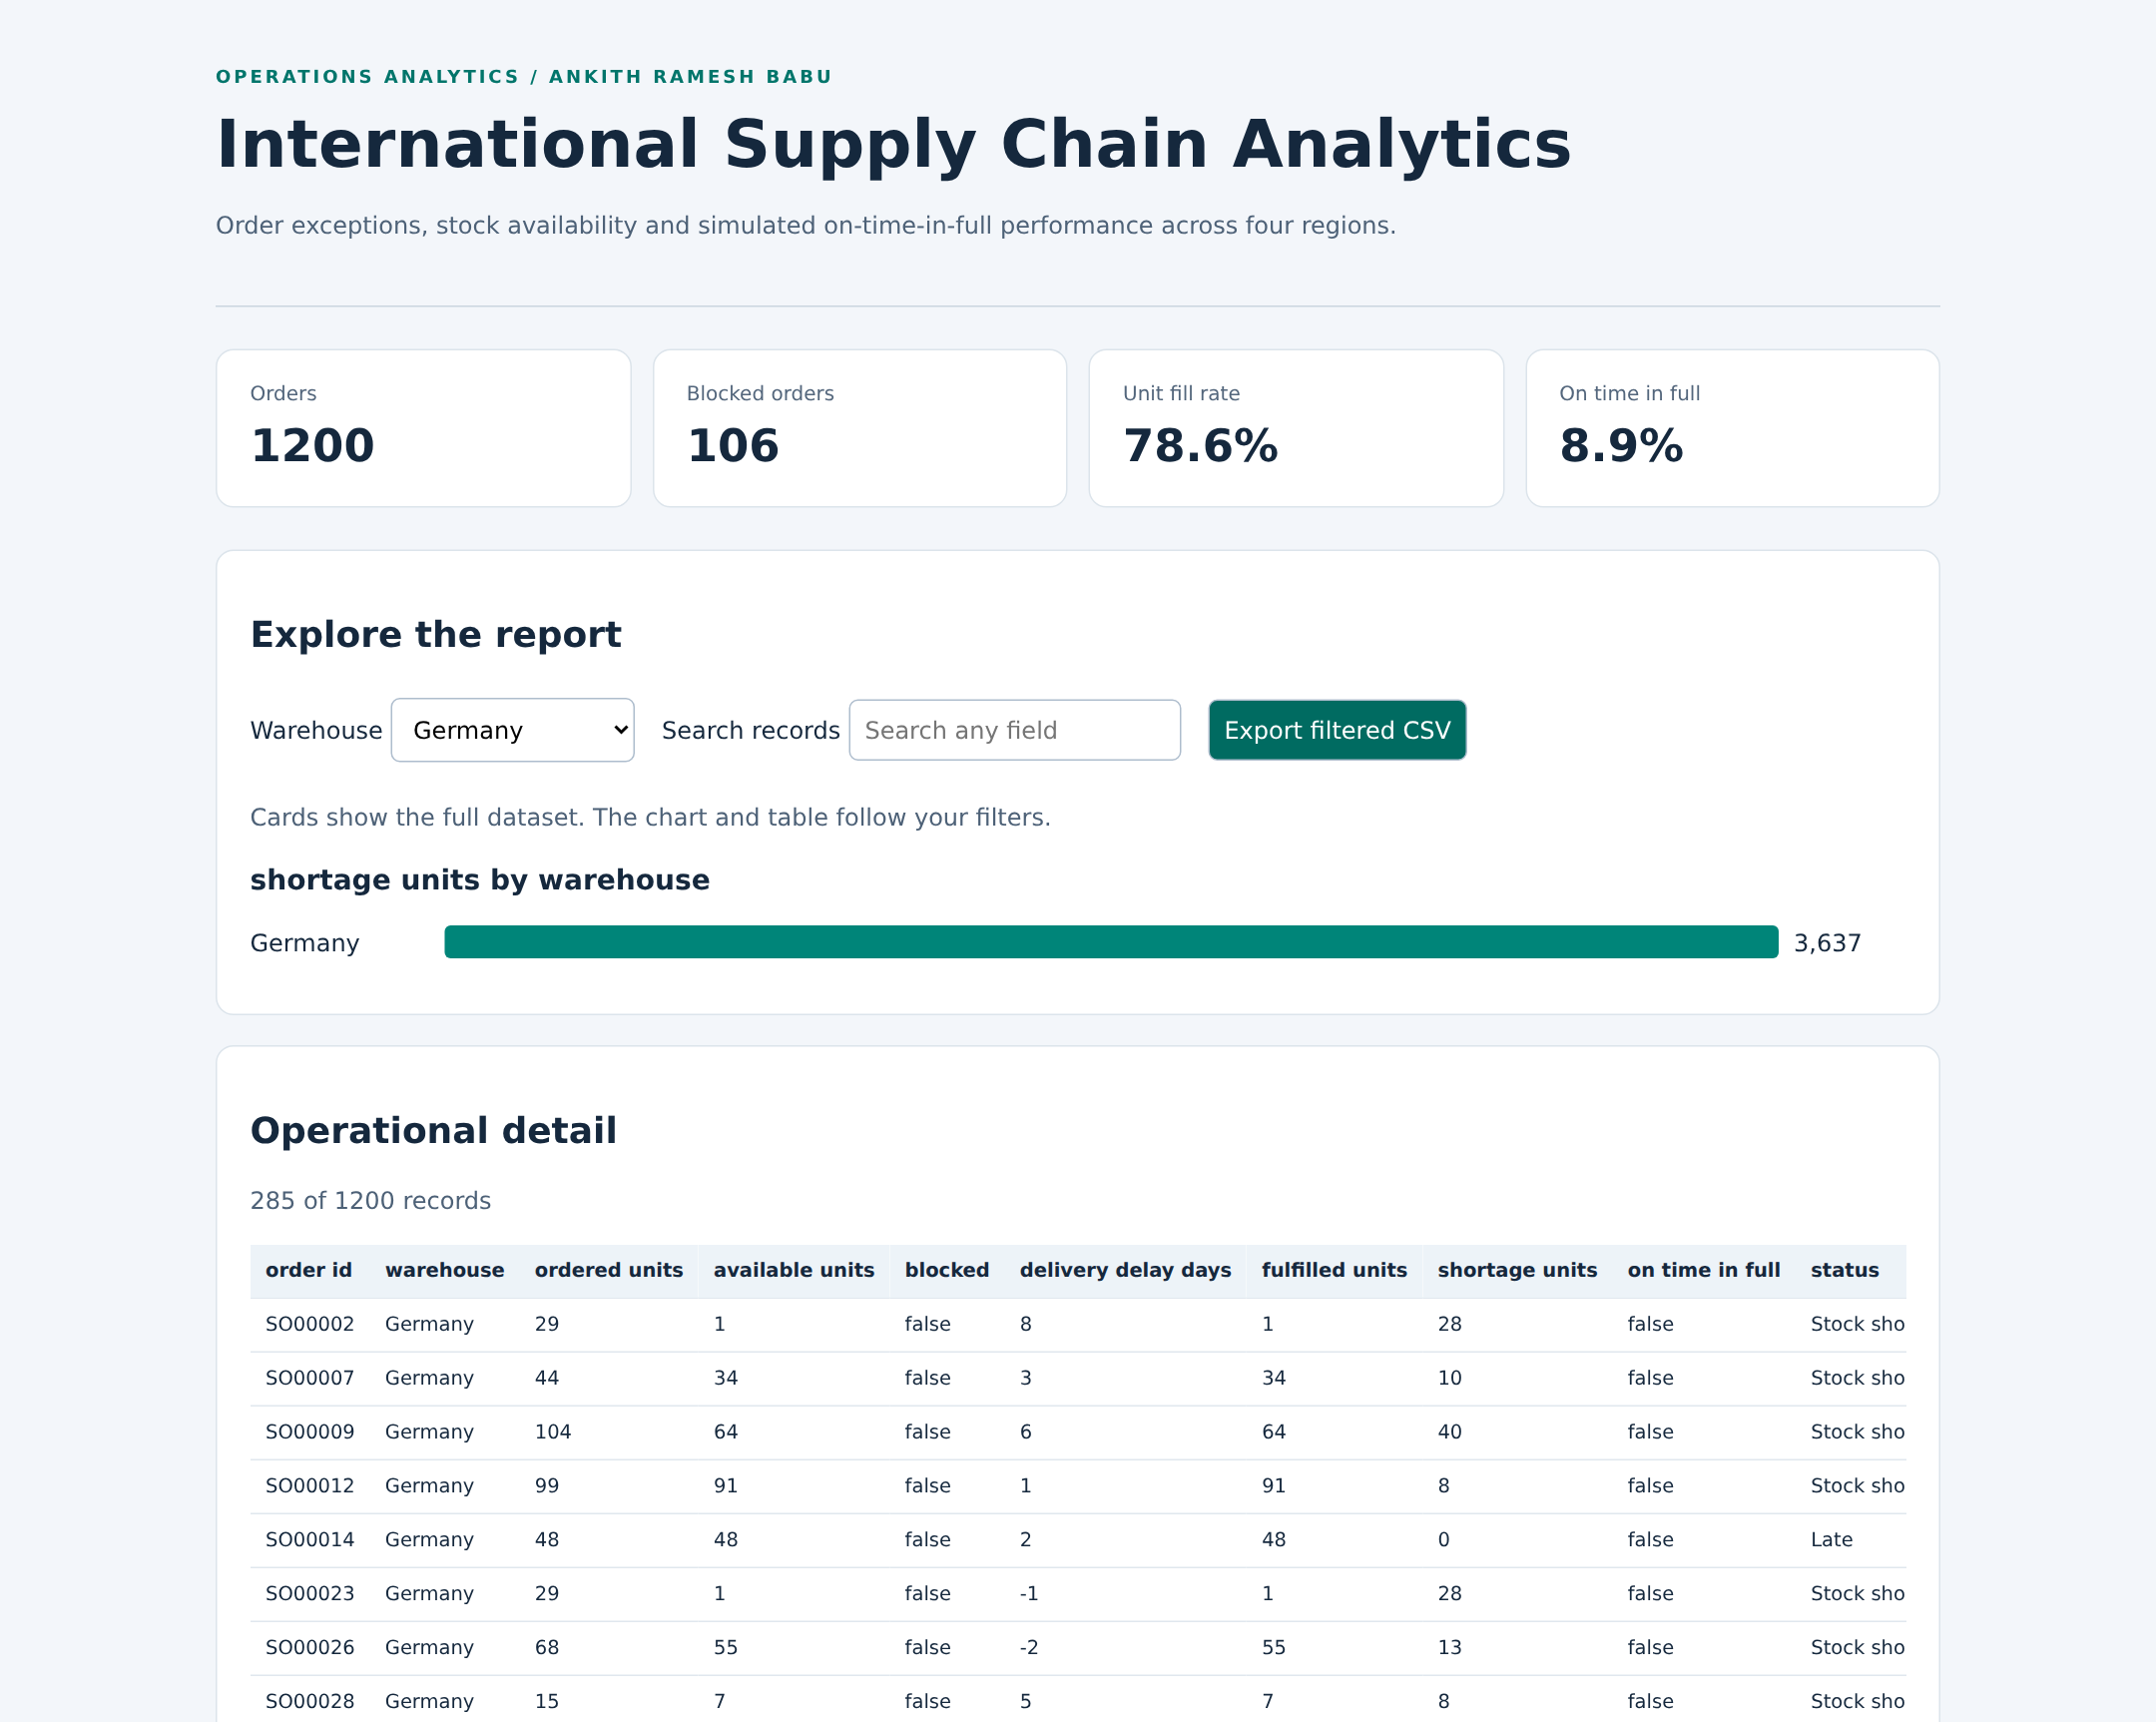
\includegraphics[width=0.90\textwidth,height=0.72\textheight,keepaspectratio]{../../reports/figures/dashboard-germany.png}
\caption{Actual browser capture with the Germany filter applied.}\label{fig:dashboard-germany}
\end{figure*}

Warehouse and search filters update the chart and visible detail rows. Summary cards intentionally remain scoped to the complete dataset. The table displays at most 200 matching rows for responsiveness. CSV export includes every matching row, not only the displayed sample.


In the browser checks, selecting Germany returned records, an unmatched search returned zero rows, and filtered CSV download succeeded. The layout also passed a 390-pixel mobile-width overflow check. The wide detail table remains horizontally scrollable.


\section{Power BI model and page layout}

The report layout is shown in Fig.~\ref{fig:powerbi-layout}.

\begin{figure*}[!t]
\centering
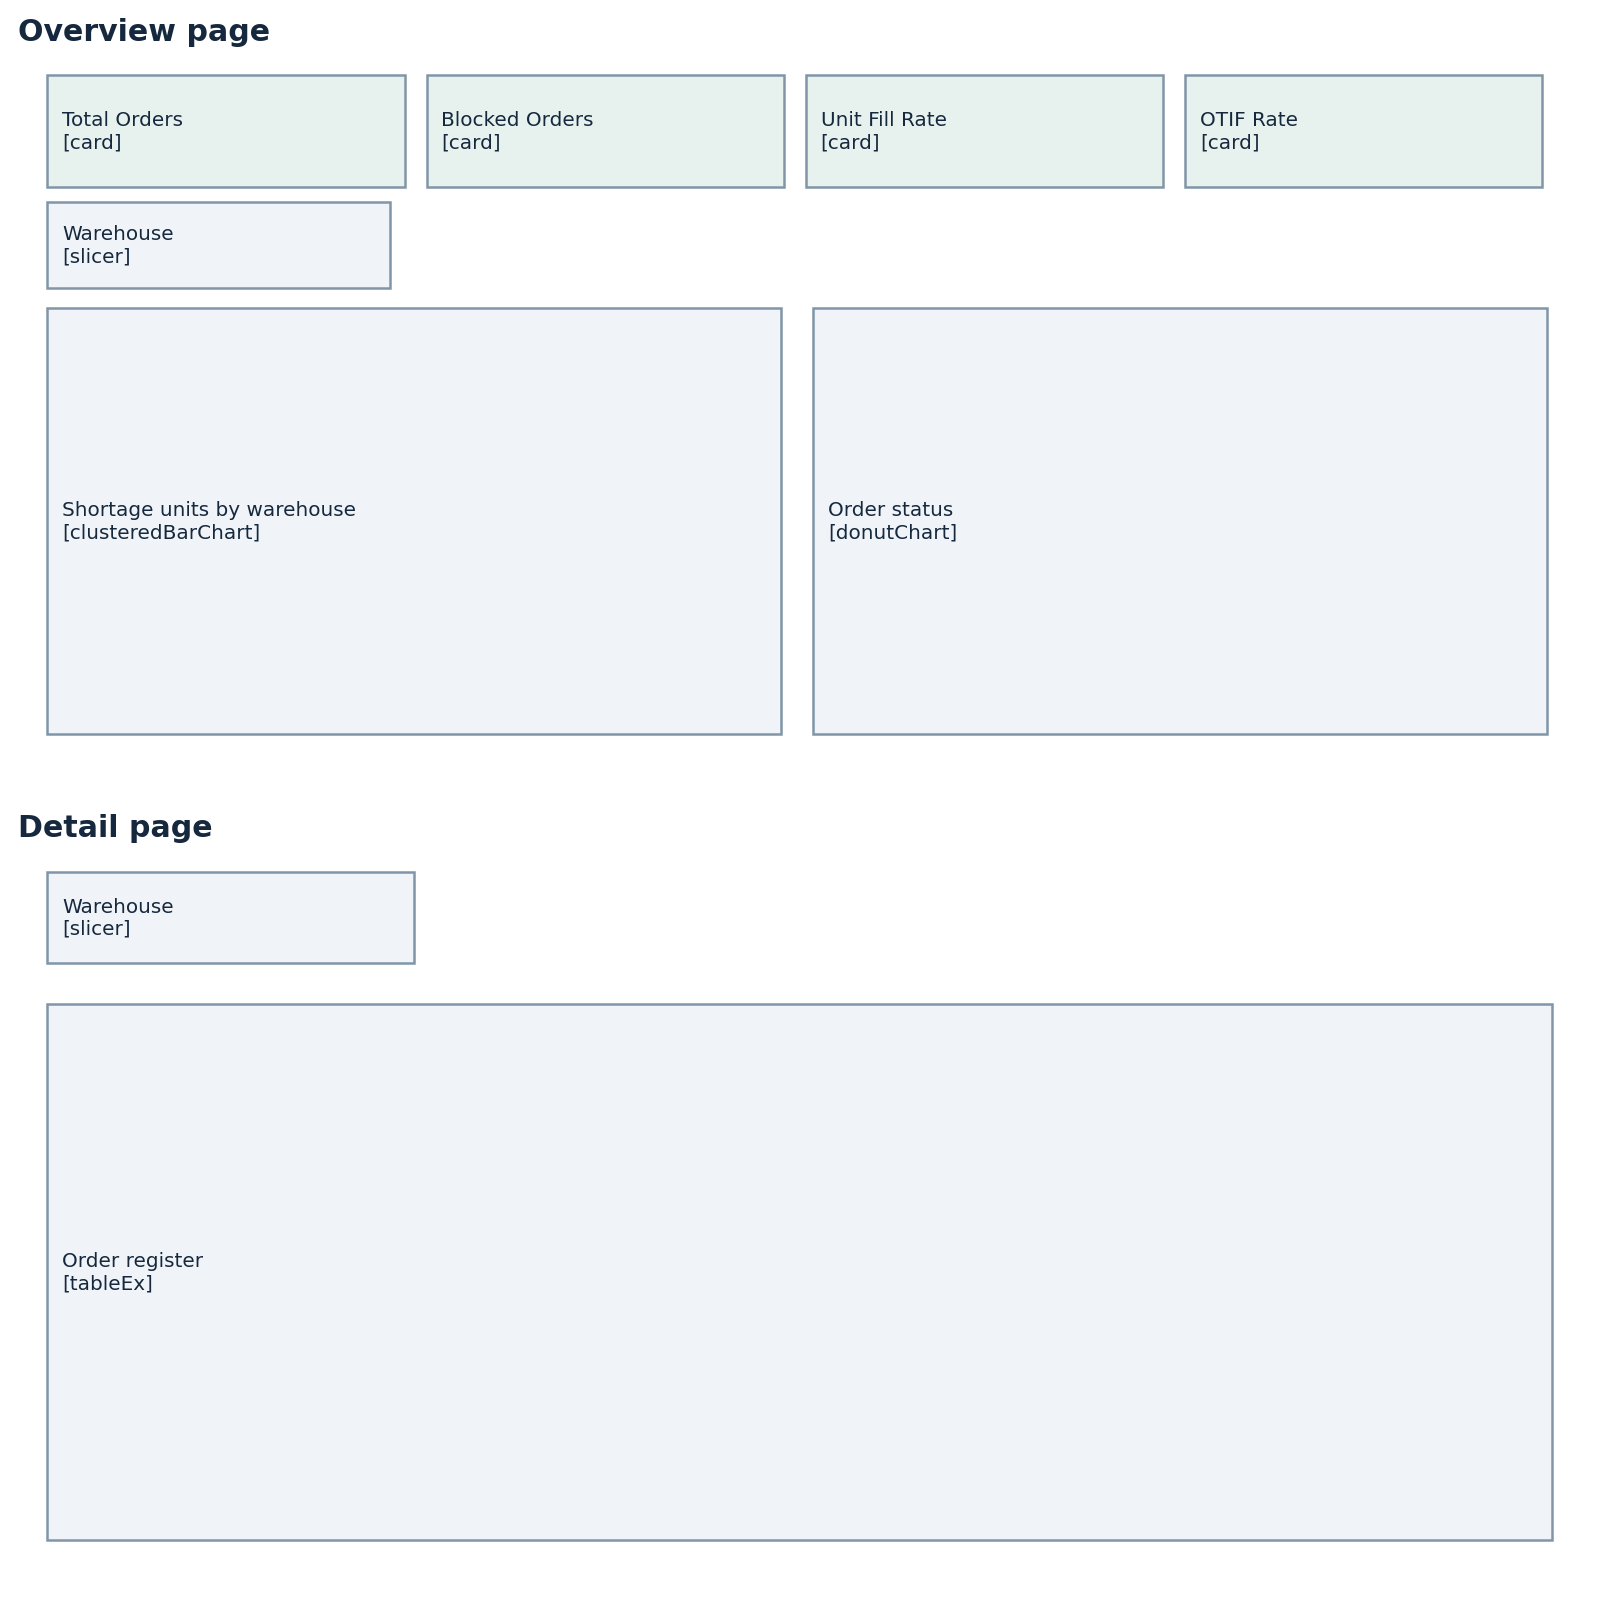
\includegraphics[width=0.90\textwidth,height=0.72\textheight,keepaspectratio]{../../reports/figures/powerbi-layout.png}
\caption{Layout diagram derived from PBIR visual coordinates. This is not a Power BI Desktop screenshot.}\label{fig:powerbi-layout}
\end{figure*}

The package includes a PBIP entry point, PBIR report pages and a TMSL model.bim semantic model \cite{r3,r4,r5}. Power Query decodes an embedded CSV snapshot, promotes headers and applies explicit data types. DAX measures provide aggregation under report filter context. Ratio measures use the DIVIDE function with an explicit alternate result for zero denominators \cite{r6}.


The overview page groups KPI cards, a warehouse slicer and two charts. The detail page exposes order-level exception fields.


Verification boundary: JSON schema and field-reference checks cover the source package. Power BI Desktop rendering, refresh and DAX execution remain outside the present validation scope. The supplied deliverable is editable Power BI project source.


\section{Sensitivity and comparative analysis}

The analysis output is shown in Fig.~\ref{fig:comparison}.

\begin{figure}[!t]
\centering
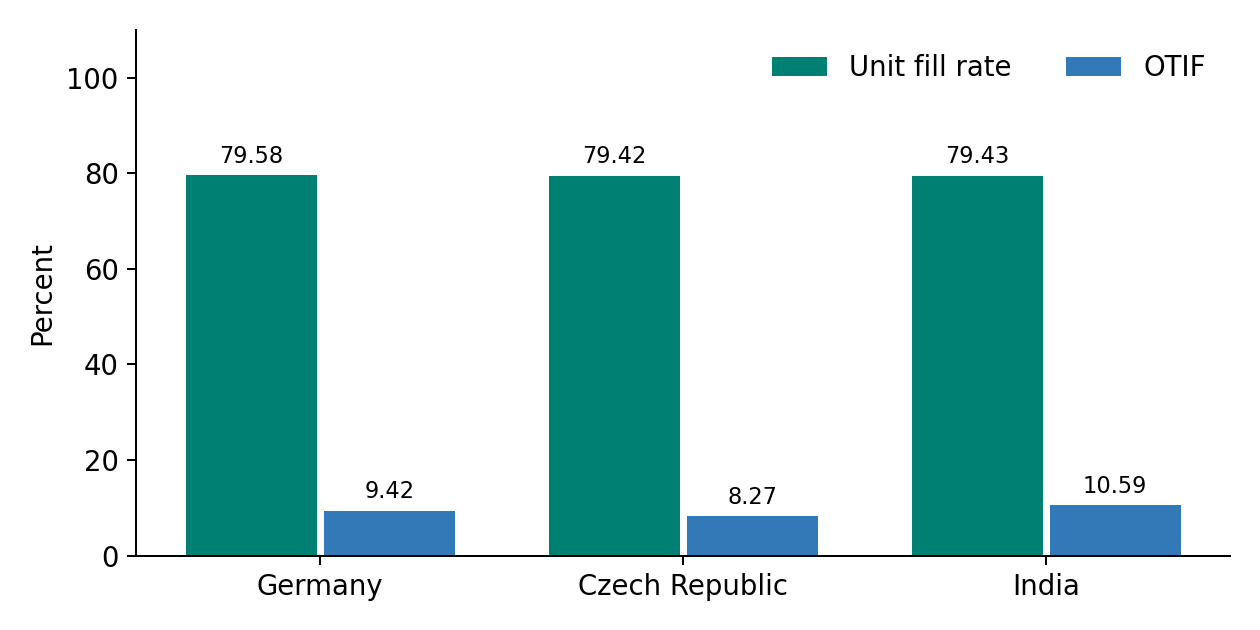
\includegraphics[width=\columnwidth,height=0.25\textheight,keepaspectratio]{../../reports/figures/comparison.png}
\caption{Warehouse-level rates under the baseline simulation.}\label{fig:comparison}
\end{figure}

Table~\ref{tab:5} summarizes sensitivity results.

\begin{table}[H]
\caption{Sensitivity results}\label{tab:5}
\centering\footnotesize
\setlength{\tabcolsep}{3pt}
\begin{tabularx}{\columnwidth}{>{\raggedright\arraybackslash}X >{\raggedright\arraybackslash}X >{\raggedright\arraybackslash}X >{\raggedright\arraybackslash}X}
\hline
\textbf{Seed} & \textbf{Blocked orders} & \textbf{Fill rate} & \textbf{OTIF} \\
\hline
7 & 127 & 78.26\% & 8.67\% \\
42 & 106 & 78.57\% & 8.92\% \\
99 & 124 & 79.32\% & 9.75\% \\
\hline
\end{tabularx}
\end{table}

The alternate-seed runs retain 1,200 orders and identical distributions. Fill rate ranges from 78.26\% to 79.32\%, while OTIF ranges from 8.67\% to 9.75\%. This checks that the analysis works beyond one random draw. It is not a statistical confidence interval or a business forecast.


The warehouse comparison reflects random allocation and sampled conditions. Ranking regions from this artificial dataset is useful for checking scorecard behavior, but not for evaluating real logistics performance.


\section{Implementation excerpts}

\subsection{KPI calculation}

\noindent\begin{minipage}{\columnwidth}
\begin{lstlisting}
def metrics(rows):
    total = sum(r["ordered_units"] for r in rows if not r["blocked"])
    filled = sum(r["fulfilled_units"] for r in rows)
    return {"orders": len(rows), "blocked_orders": sum(r["blocked"] for r in rows),
            "fill_rate": round(filled / total, 4) if total else 0,
            "otif_rate": round(sum(not r["blocked"] and r["fulfilled_units"] == r["ordered_units"] and r["delivery_delay_days"] <= 0 for r in rows) / len(rows), 4) if rows else 0}

\end{lstlisting}
\end{minipage}


The denominator explicitly excludes blocked orders for unit fill rate. OTIF requires all three conditions in a single predicate. Empty input produces zero rather than a division error. The DAX DIVIDE measure applies the same zero-denominator policy \cite{r6}.


\subsection{Power BI measure}

\noindent\begin{minipage}{\columnwidth}
\begin{lstlisting}
OTIF Rate =
DIVIDE(
  CALCULATE(COUNTROWS(orders),
            orders[on_time_in_full] = TRUE()),
  COUNTROWS(orders),
  0
)
\end{lstlisting}
\end{minipage}


\subsection{Code organization}

src/run.py owns simulation and business rules. src/reporting.py handles CSV and HTML rendering. scripts/analyze.py creates scenario evidence. scripts/build\_powerbi.py regenerates the embedded snapshot and report definitions. Tests exercise calculations, edge cases and report generation.


\section{Validation and reproducibility}

Table~\ref{tab:6} summarizes verification evidence.

\begin{table}[H]
\caption{Verification evidence}\label{tab:6}
\centering\footnotesize
\setlength{\tabcolsep}{3pt}
\begin{tabularx}{\columnwidth}{>{\raggedright\arraybackslash}X >{\raggedright\arraybackslash}X >{\raggedright\arraybackslash}X}
\hline
\textbf{Check} & \textbf{Evidence} & \textbf{Outcome} \\
\hline
Business-rule tests & Blocked/partial OTIF, quantity bounds and invalid counts & Passed \\
Repeat generation & Same seed and arguments reproduce identical exports & Passed \\
Browser interactions & Warehouse filter, empty search, CSV export, mobile width & Passed \\
Report source & PBIR JSON schema and model-field linkage checks & Passed \\
Desktop Power BI & Windows application, refresh and DAX engine & Not executed \\
\hline
\end{tabularx}
\end{table}

\subsection{Reproduction commands}

\noindent\begin{minipage}{\columnwidth}
\begin{lstlisting}
python src/run.py
python scripts/analyze.py
python scripts/build_powerbi.py
python -m unittest discover -s tests -v
\end{lstlisting}
\end{minipage}


The default analysis uses the Python standard library. The report is compiled from the included IEEEtran LaTeX source using pdfLaTeX. PDF charts and tables draw from committed CSV and JSON outputs. Browser screenshots record the generated HTML interface rather than a hand-drawn imitation.


\subsection{Cross-checks}

The total primary-status count equals 1,200. Fulfilled units never exceed ordered or available units. Blocked orders always have zero fulfillment. The exception export contains only non-On track rows. The scorecard partitions the same order population.


\subsection{Scope of assurance}

Passing these checks establishes internal consistency for the stated rules and dataset. It does not establish calibration against a real warehouse, production readiness or economic benefit.


\section{Limitations and conclusion}

\subsection{Model limitations}

\textbullet{} Stock snapshots are independent across orders, so orders do not compete for a shared balance.


\textbullet{} Delay and block status are independently sampled. Real causes are often correlated.


\textbullet{} No promised calendar date, transport milestone or partial-shipment history exists.


\textbullet{} The scenario analysis changes random seeds rather than estimating real uncertainty.


\subsection{Next engineering priorities}

An operational extension should introduce validated external data, explicit business definitions, schema checks and exception ownership. A continuous stock ledger and dated shipment events would enable a more realistic service model.


\subsection{Conclusion}

The project provides an auditable chain from simulated observations to decision fields, exports and visual review. Its main contribution is a consistent separation of fulfillment, strict OTIF and exception priority.


The reported outputs are reproducible and the calculation boundaries are documented. Power BI source is supplied as an editable project, with Desktop verification explicitly separated from the automated source checks.


\section{Artifact Availability}

\subsection{Artifact index}

Table~\ref{tab:7} summarizes repository artifacts.

\begin{table}[H]
\caption{Repository artifacts}\label{tab:7}
\centering\footnotesize
\setlength{\tabcolsep}{3pt}
\begin{tabularx}{\columnwidth}{>{\raggedright\arraybackslash}X >{\raggedright\arraybackslash}X}
\hline
\textbf{Path} & \textbf{Purpose} \\
\hline
src/ & Simulation, calculations and HTML reporting \\
reports/*.csv, *.json & Baseline and scenario evidence \\
reports/dashboard.html & Interactive operational dashboard \\
reports/figures/ & Actual browser captures, charts and layout diagram \\
powerbi/ & PBIP, PBIR and semantic model source \\
tests/ & Automated checks \\
docs/methodology.md & Definitions and assumptions \\
reports/project-report.pdf & This technical report \\
\hline
\end{tabularx}
\end{table}

\balance
\begin{thebibliography}{00}

\bibitem{r1} Python Software Foundation. random: Generate pseudo-random numbers. [Online]. Available: \url{https://docs.python.org/3/library/random.html}. Accessed: Oct. 27, 2026.


\bibitem{r3} Microsoft. Power BI Desktop projects. [Online]. Available: \url{https://learn.microsoft.com/en-us/power-bi/developer/projects/projects-overview}. Accessed: Oct. 27, 2026.

\bibitem{r4} Microsoft. Power BI project report folder and PBIR. [Online]. Available: \url{https://learn.microsoft.com/en-us/power-bi/developer/projects/projects-report}. Accessed: Oct. 27, 2026.

\bibitem{r5} Microsoft. Power BI project semantic model folder. [Online]. Available: \url{https://learn.microsoft.com/en-us/power-bi/developer/projects/projects-dataset}. Accessed: Oct. 27, 2026.

\bibitem{r6} Microsoft. DIVIDE function (DAX). [Online]. Available: \url{https://learn.microsoft.com/en-us/dax/divide-function-dax}. Accessed: Oct. 27, 2026.

\end{thebibliography}
\end{document}
